\section{Anhang}
\subsection{Netz Laborversuch}
\begin{table}[H]
\begin{tabular}{|c|c|}
\hline 
\textbf{Bezeichnung} & \textbf{Netz 1} \\ 
\hline 
Kurzschlussleistung $S_k''$ & 1000MVA \\ 
\hline 
Kurzschlussleistung $S_k''$ Maximum & 1000 \\ 
\hline 
Kurzschlussleistung $S_k''$ Minimum & 1000 \\ 
\hline 
Verhältnis R/X & 0.1 p.u. \\ 
\hline
\end{tabular} 
\caption{Nenndaten des starren Netzes}
\end{table}

\begin{table}[H]
\begin{tabular}{|c|c|c|}
\hline 
\textbf{Bezeichnung} & \textbf{Transformator 1} & \textbf{Transformator 2} \\ 
\hline 
Nennspannung Seite 1 $U_{n1}$ & 110kV & 110kV \\ 
\hline 
Nennspannung Seite 2 $U_{n2}$ & 10kV & 10kV \\ 
\hline 
Nennscheinleistung $S_n$ & 100MVA & 80MVA \\ 
\hline 
Dauerleistung $S_{max}$ & 100MVA & 80MVA \\ 
\hline 
Kurzschlussspannung $u_k$ & 12\% & 12\% \\ 
\hline 
Ohmsche Kurzschlussspannung $u_r$ & 0,38\% & 0,38\% \\ 
\hline 
Schaltgruppe & Yy0 & Yy0 \\ 
\hline 
\end{tabular}
\caption{Nenndaten Transformatoren}
\end{table}

\begin{table}[H]
\begin{tabular}{ll}

\begin{tabular}{|c|c|}
\hline 
\textbf{Bezeichnung} & \textbf{Kenndaten} \\ 
\hline 
Leitungstyp & Freileitung \\ 
\hline 
Widerstand r & 0,118 Ohm/km \\ 
\hline 
Reaktanz x & 0,421 Ohm/km \\ 
\hline 
Kapazität c & 9,17nF/km \\ 
\hline 
Nennspannung & 110kV \\ 
\hline 
Therm. Grenzstrom & 645A \\ 
\hline 
\end{tabular}

&

\begin{tabular}{|c|c|}
\hline 
\textbf{Leitung} & \textbf{Länge} \\ 
\hline 
L12 & 30km \\ 
\hline 
L16 & 50km \\ 
\hline 
L23 & 45km \\ 
\hline 
L25 & 30km \\ 
\hline 
L34 & 25km \\ 
\hline 
L45 & 20km \\ 
\hline 
L64 & 35km \\ 
\hline 
L67 & 20km \\ 
\hline 
\end{tabular}

\end{tabular}

\caption{Freileitungen}
\end{table}

\begin{table}[H]
\begin{tabular}{|c|c|c|}
\hline 
\textbf{Last} & \textbf{Scheinleistung} & \textbf{Leistungsfaktor} \\ 
\hline 
Last 1 & 40MVA & 0,95 \\ 
\hline 
Last 2 & 30MVA & 0,8 \\ 
\hline 
Last 3 & 60MVA & 0,9 \\ 
\hline 
Last 5 & 40MVA & 0,9 \\ 
\hline 
Last 7 & 60MVA & 0,9 \\ 
\hline 
\end{tabular}
\caption{Lasten}
\end{table}

\begin{table}[H]

\begin{tabular}{|l|c|c|}
\hline 
\textbf{Bezeichnung} & \textbf{Generator 1} & \textbf{Generator 2} \\ 
\hline 
Maschinentyp & Turbogenerator & Turbogenerator \\ 
\hline 
Bemessungsscheinleistung & 100MVA & 80MVA \\ 
\hline 
Bemessungsspannung & 10kV & 10kV \\ 
\hline 
Verhältnis R/X & 0,1 p.u. & 0,1 p.u. \\ 
\hline 
Anlaufzeitkonstante $T_A$ & 8,2s & 8,2s \\
\hline
Gleichstromzeitkonstante $T_G$ & 0,36s & 0,36s \\
\hline
Ankerwiderstand $R_a$ & 0,01 p.u. & 0,01 p.u. \\
\hline
Ankerstreureaktanz $X_{1\sigma}$ & 0,13 p.u. & 0,13 p.u. \\
\hline
\multicolumn{3}{|l|}{Kurzschlusszeitkonstanten} \\
\hline
• subtransient d-Achse $T_d''$ & 0,03s & 0,03s \\
\hline
• subtransient q-Achse $T_q''$ & 0,03s & 0,03s \\
\hline
• transient d-Achse $T_d'$ & 1,0s & 1,0s \\
\hline
• subtransient q-Achse $T_q'$ & 1,0s & 1,0s \\
\hline
\multicolumn{3}{|l|}{Reaktanzen} \\
\hline
• subtransient d-Achse $X_{d}''$ & 20\% & 20\% \\ 
\hline
• subtransient q-Achse $X_q''$ & 20\% & 20\% \\
\hline
• transient d-Achse $X_{d}''$ & 30,1\% & 30,1\% \\ 
\hline
• transient q-Achse $X_q''$ & 100\% & 100\% \\
\hline
• stationär d-Achse $X_d$ & 227\% & 227\% \\
\hline
• stationär q-Achse $X_q$ & 205\% & 205\% \\
\hline
Bemessungsleistungsfaktor & 0,9 & 0,9 \\ 
\hline 
Wirkleistung P & 90MW & 72MW \\ 
\hline 
Generatorspannung & 10kV & 10kV \\ 
\hline
\end{tabular}

\caption{Generatoren}
\end{table}


	\begin{figure}[H]
	\centering
	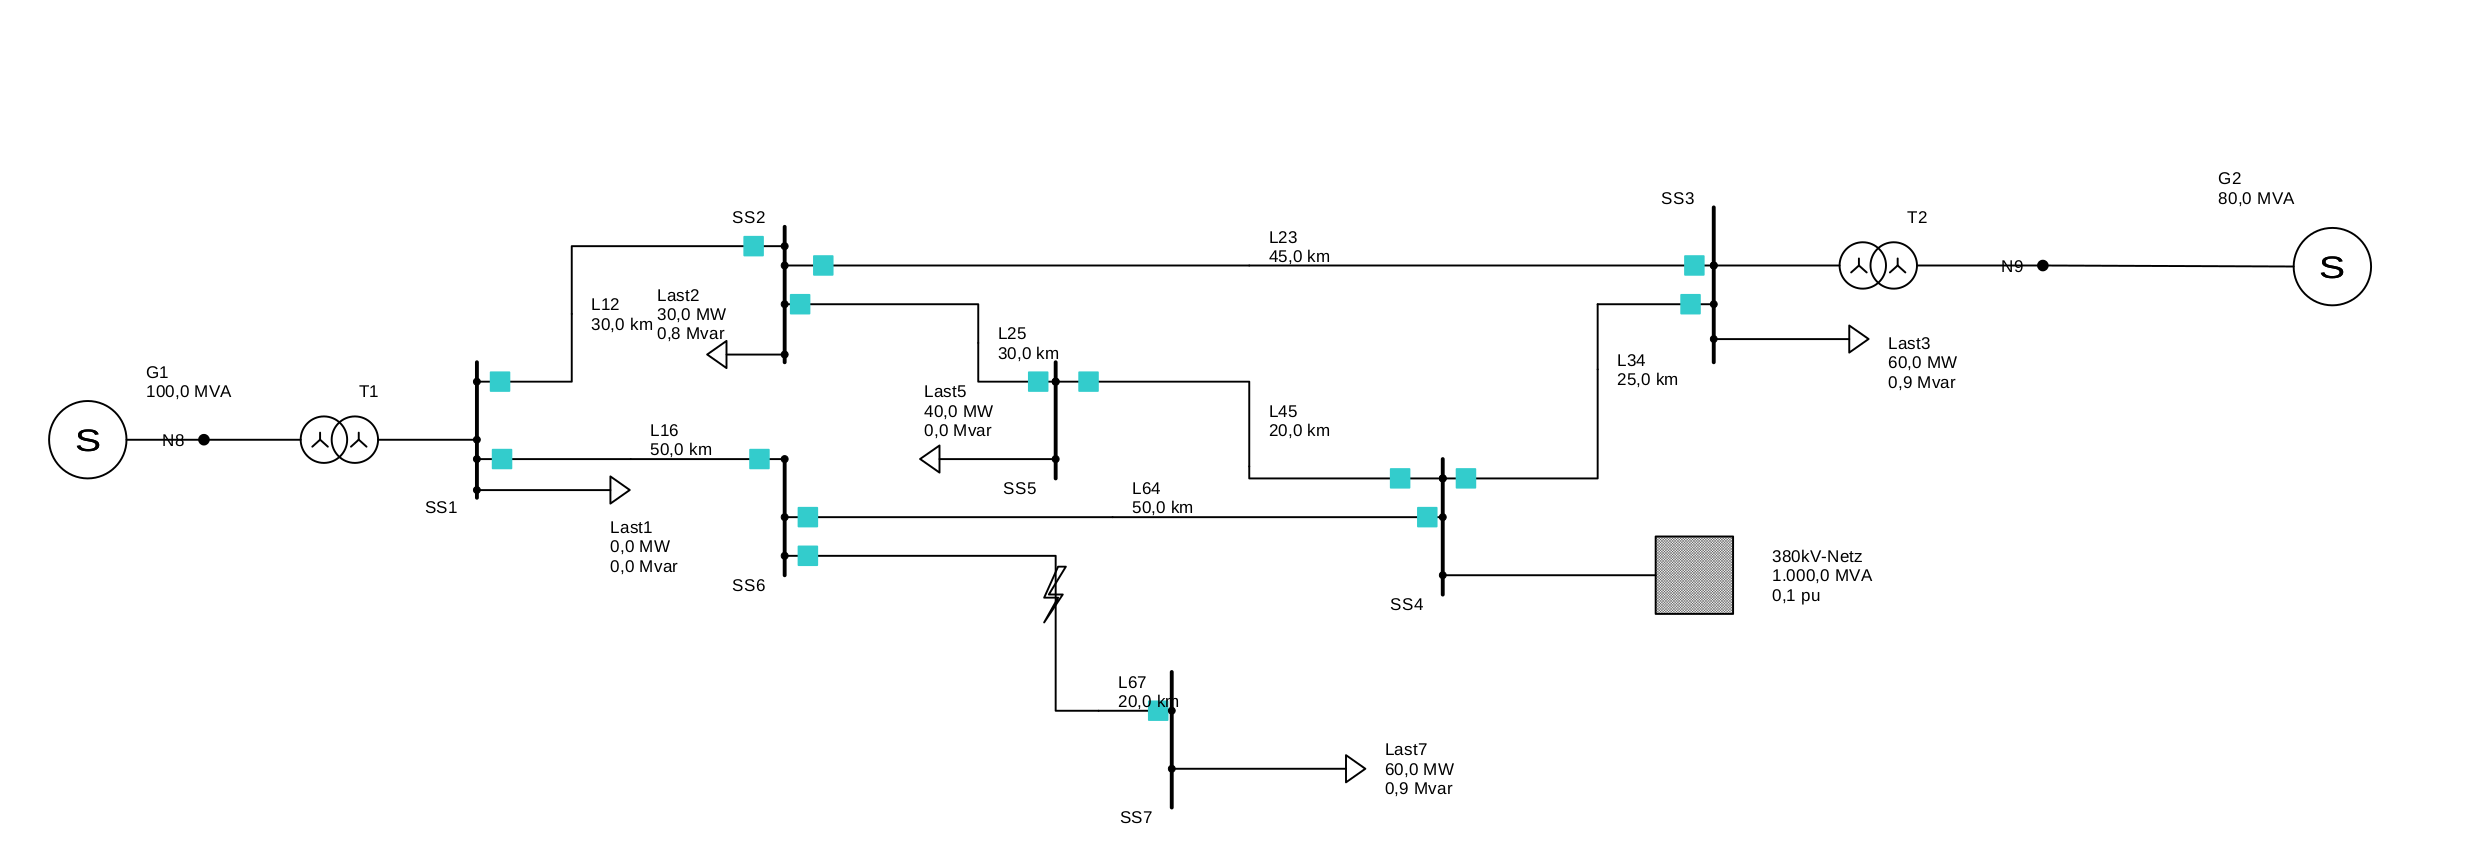
\includegraphics[scale=0.35, angle=90]{img/praktikum-netz}
	\caption{Netzaufbau Laborversuch}
	\label{praktikum-netz}
	\end{figure}